%%%%%%%%%%%%%%%%%%%%%%%%%%%%%%%%%%%%%%%%%%%%
% PRODUCING A SELF-DRIVING MODEL
%%%%%%%%%%%%%%%%%%%%%%%%%%%%%%%%%%%%%%%%%%%%

\section{Producing a self-driving model}


% probably best to more this to results section and reference here
%\begin{verbatim}
%# data: genRoad (log2 renamed)
%# commit: 1ad187d4bff5b6936c065a1aaa15a654ef4d368c
%$ python train.py --model=sanity --outdir=../trained_models
%\end{verbatim}
%this will create the a model in trained\_output/sanity/20201120184912\_sanity.h5
% and run as per procedure described in (TODO add reference).
More results, this time as per run 43 (\ref{app_res:43}) 3 images side by side (Figure 
 \ref{fig:tcpflow_Run43}). This was a first attempt to add rain, where the effect is added to the image presented to network. Although the procedure introduces noise to images, it is somewhat unrealistic, as rain is expected to be present on the acquired image. It is left here to document the work development.
 
\begin{figure}[ht]
 \centering 
 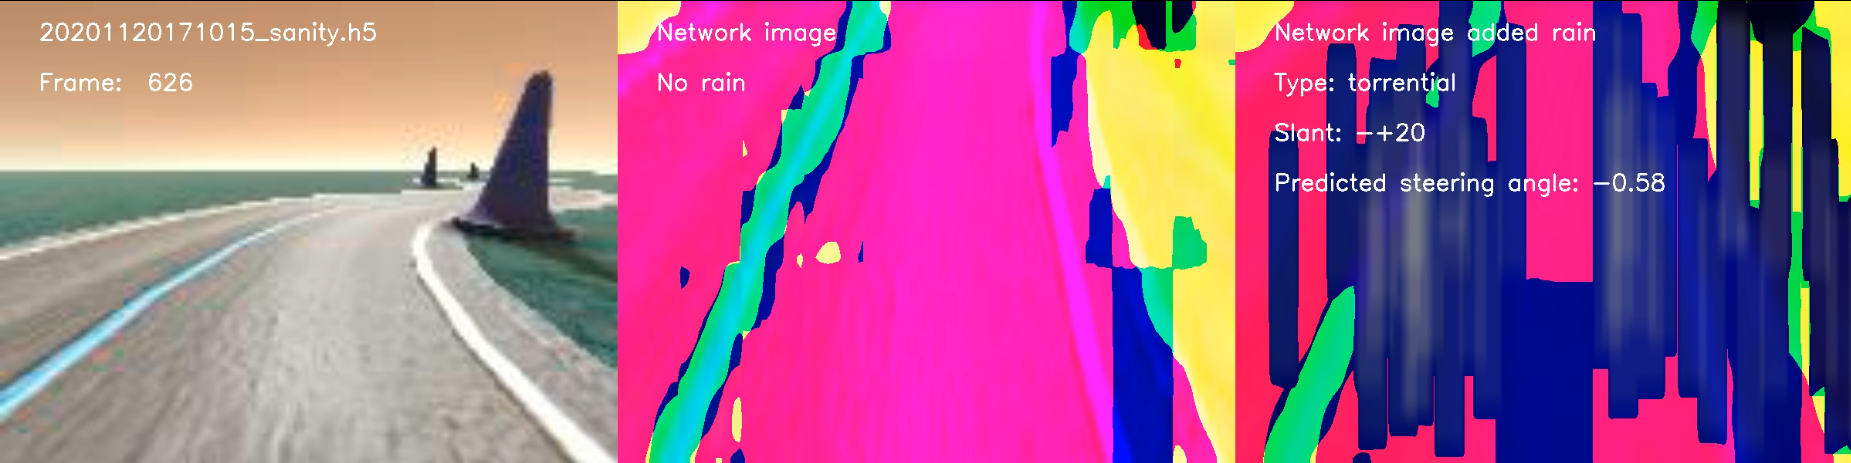
\includegraphics[width=\textwidth]{Figures/tcpflow_Run43.png}
 \caption{Video still showing torrential rain added to the image presented to the network \href{https://youtu.be/57jwwcjbfdE}{https://youtu.be/57jwwcjbfdE}}
 \label{fig:tcpflow_Run43} 
\end{figure}
%\begin{verbatim}
%# data: genRoad (log2 renamed)
%# commit: 1ad187d4bff5b6936c065a1aaa15a654ef4d368c
%$ python train.py --model=sanity --outdir=../trained_models
%\end{verbatim}
%this will create the a model in trained\_output/sanity/20201120184912\_sanity.h5
%and run as per procedure described in (TODO add reference).

\section{Producing a self-driving model}
A self-driving model that successfully drove around the Generated Track was produced 


TODO describe how SDSandbox did not work out of the box - author mentions in video "several hours of data are required" and model to nearly 24 hours to train on GPU. In practice, one augmentation and pre-processing were added, working models were produced in as little as 5 epochs of training, taking under 1m30s.
That was hard. Detail the bits that were used from TawnNet (augmentation added) and NaokiNet (crop changed). in the end two outputs were required for NaokiNet to work. Maybe move this to discussion. Here we show results.

%%%%%%%%%%%%%%%%%%%%%%%%%%%%%%%%%%%%%%%
% NETWORK TRAINING
%%%%%%%%%%%%%%%%%%%%%%%%%%%%%%%%%%%%%%%

\section{Network training and simulator testing}
\label{results:net-training} 
% write up, label runs and make reference
The first working model (able to successfully self-drive around the Generated Track) was 20201107210627\_ nvidia1.h5. A video was generated using the recording screen utility Kazam (\cite{Kazam2020}), recording at 15fps (frames per second), and published at  \href{https://youtu.be/9z0mMtOnUUc}{https://youtu.be/9z0mMtOnUUc}. Figure \ref{fig:SimTCPPred}
shows 3 stills from the video containing from left to right, the game engine, the TCP debug output and the prediction engine running.

\begin{figure}[h!]
\centering
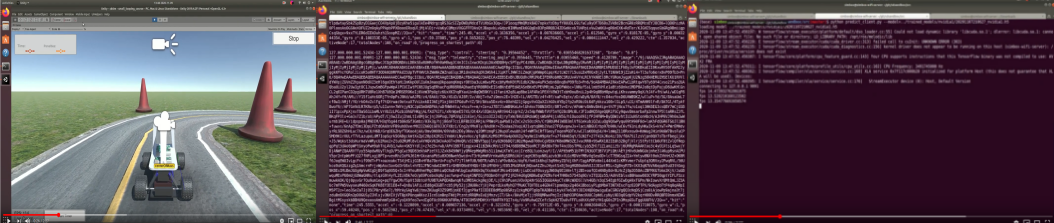
\includegraphics[width=\textwidth]{Figures/SimTCPPred.png}
\caption{Stills of video \href{https://youtu.be/9z0mMtOnUUc}{https://youtu.be/9z0mMtOnUUc} showing left to right: SDSandbox simulated car going around the Generated Track course, TCP Debug (tcpflow) and prediction engine (predict\_ client.py) running}
\label{fig:SimTCPPred}
\end{figure}

The video shows the TCP debugging, prediction engine and the game engine simulated car steering with predictions received over the TCP network. The actual code used to generate the model was not logged at the time the experiment log entry was written in the appendix log (\ref{AppendixD}). By verifying git hash commits (4 commits were made on November 7th) as documented in appendix  a second sanity check model \ref{app_res:36} (20201120171015\_ sanity.h5) was created and found to self-drive successfully around the generated track. A video was made from tcpflow frames as described at the end of \ref{app_res:36}, and uploaded to \href{https://youtu.be/JaSkkh-2xtI}{https://youtu.be/JaSkkh-2xtI}.
The video shows (fps discrepancies considered) that the \ref{app_res:36} model had a better lap around the track.
Model 37 (\ref{app_res:37}) trained with genRoad (including outliers seen in Figure \ref{fig:GeneratedRoadPlusHist}) ) did not do well. The oversteering can be seen in video \href{https://youtu.be/xGDN8qOnv9M}{https://youtu.be/xGDN8qOnv9M}. The steering angle bins and graph plots can be seen in  Figures \ref{fig:tcpflow_20201120184912_bins}  and \ref{fig:tcpflow_20201120184912_graph} in the results appendix.

% a number of runs (e.g. commit 2e5bf1b7 failed prematuraly, most failing to generate a model. Doing a diff on one of them shows that batch size was set to 128
% Could this also be an issue?
% Note in original Alexnet which we assume NVIDIA were using as a design reference, used batch size 128 for TWO channels - TODO write-up in Discussion.

%$ git diff master..2e5bf1b7 train.py | grep batch_size
%-    batch_size = conf.batch_size
%+    batch_size = conf.training_batch_size
%(base) simbox@simbox-wifi-server:~/src(master)$ git diff master..2e5bf1b7 conf.py | grep %batch_size
%+training_batch_size = 128
%-batch_size = 64
%+batch_size = 128 # nvidia1 = 64
%@@ -50,7 +49,5 @@ batch_size = 64


Another set of results for the best performing nvidia2 architecture. TODO ADD DISCUSSION, nearly steering off at large negative spike - link to video time, for three videos.  

(\url{https://youtu.be/qdTA5ho5VOE}) shows a still containing three images. The tcpflow log captured when the video was recorded provided data to plot the orange line (intensity multiplier 4, light rain) in Figure \ref{fig:sa_GeneratedTrackintensitymultiplier4_20201207091932_nvidia1}. The vehicle steers off the road and fails to turn right.


%%%%%%%%%%%%%%%%%%%%%%%%%%%%%%%%%%%%%%%%%
% DATA GATHERING
%%%%%%%%%%%%%%%%%%%%%%%%%%%%%%%%%%%%%%%%%
TODO git diff (in appendix) and itemize modifications.
    
Models are trained with code written in train.py, models.py and conf.py. This code has been modified from the original. To compare changes a git diff can be copying the original code over the source code used in this project and performing a "git diff"
\begin{verbatim}
# clone repository for dissertation
$ git clone https://github.com/dsikar/sdsandbox
# clone original
$ git clone https://github.com/tawnkramer/sdsandbox sandbox_orig
# copy original over dissertation
$ cp sandbox_org/src/* sdsandbox/src
# compare
$ cd sdsandbox 
$ git diff
\end{verbatim}


Starting with the NVIDIA baseline, a number of hyperparameters were trialed. The initial setup failed to generate usable models. 
The table below presents training results for best trained models.



Using the baseline neural network architecture as described in 
Models trained with no image pre-processing, did not perform well, leading to cars driving off the road, as shown in Fig.  sequence.

% data gathered on Robot Racing League track
We gathered 10 laps of data on the Robot Racing League track, with maximum speed set to 2.1, proportional control set to 16 and differential set to 77. Maximum steer was set to 25 (degrees). Corresponding to 12778 .jpg image files and the same number of  .json files, containing corresponding throttle and steering angle values recorded at the moment image was saved by simulator. This can be seen in the calls to Update() and SaveCamSensor functions in  
\begin{verbatim}
./Assets/Scripts/Logger.cs
\end{verbatim}


% Best performing NVIDIA model

Figure \ref{fig:20201207192948_nvidia2_mult_1_4_8_light} shows 3 stills taken for corresponding videos of network nvidia2 20201207192948\_ nvidia2.h5 (best performing model in the rain), for runs 83 (\ref{app_res:83}), 86 (\ref{app_res:86}) and 89 (\ref{app_res:89}), containing from left to right, the acquired image as produced by the Unity3D game engine (SDSandbox), the same image with added light rain and the processed image as presented to the network, which then predicts a steering angle. The first row for intensity multiply 1, the second for 4 and the third for 8. There are no lane markings in the last row, suggesting the network has learned about road boundaries and is able to generalise, given the image being presented (no lane markings) had never been seen before.

%%%%%%%%%%%%%%%%%%%%%%%%%%%%%%
% RESULTS REMOVED
%%%%%%%%%%%%%%%%%%%%%%%%%%%%%%

Discuss:
\begin{itemize}
    \item[--] Validity
    \item[--] Scope
    \item[--] Generalisability
    \item[--] Implications
    \item[--] Recommendations
\end{itemize}
Havoc created by outliers in genRoad. 20201206211122\_ nvidia1.h5 performs well on genRoad (where is was trained) but not well on genTrack. Models trained on genTrack also do well on genRoad. Why?
TODO On previous note, add Run 95 - over 16 minute drive \url{https://youtu.be/z9nILq9dQfI}  
Discuss how results in Table \ref{table:goodness-of-steer} fail to indicate numerically that nvidia2 was better than nvidia1 in the rain. A windowing approach may be required, to identify "spikes" to quantify a "crash" likelyhood. The quantity does confirm what has been observed through qualitative analysis, that nvidia2 is a "smoother" drive.  
TODO Add observation on Why
TODO Add note on base data causing model to misbehave
TODO Add How Outliers messed up training
Todo add The code used to generate the model was not logged at the time. Some forensics conducted in \ref{app_res:36}
Todo Add Run 3 - one output, bad result.
TODO Video not recorded for ground truth in figures 1.12 through 1.14, left tcpflow log in /tmp folder, deleted after reboot.

%%%%%%%%%%%%%%%%%%%%%%%%%%%%%%%
% EVALUATION
%%%%%%%%%%%%%%%%%%%%%%%%%%%%%%%

his section discussed the evaluation benchmarks, here we discuss the evaluation environment (Unity 3D game engine) and how it was used to both generate data and evaluate the models.
We have so far a goodness of steer metric. Additionally, it would be good to have some form of noise measure, to quantify how much the image has been changed by random noise, i.e. rain.



To generated predictions \textit{on-the-fly}, the simulator is run in \textit{Auto Drive w Rec} mode. Once activated, the sends frames over the network using the OpenAI Gym (\cite{brockman2016openai} (TODO FURTHER DISCUSS PLATFORM) framework which sends packets over the network. The packets are sent from simulator using TCP (\cite{rfc793}), include packets \textbf{DESCRIBE PACKETS}.  
\textbf{DESCRIBE HANDSHAKING} \textbf{DESCRIBE TCP} 
\textbf{DESCRIBE GRAPH}
Figure \ref{fig:PredSteeringAnglestcpflowNvidia1} shows a plot of predicted and simulator steering angles. The prediction is for a single image frame sent over the network. As the simulation begins, frames are sent over the network and in this case, captured with tcpflow (\cite{garfinkel2013passive}. A log file was produced. The log file was processed (\cite{JUPYTERNOTEBOOKINAPPENDIX} and created plot. This was for one lap of the \textit{Generated Track}, similar to the track shown in Figure \ref{fig:GeneratedTrackPlusHist}. The actual processing frame rate is approximately 11fps. The y axis is flipped so the plot relates to the path taken by simulated vehicle, the first drop indicating the first right turn, the rise and sharp drop indicating the sharp right turn at the opposite end of the starting line.

\begin{figure}[ht]
 \centering 
 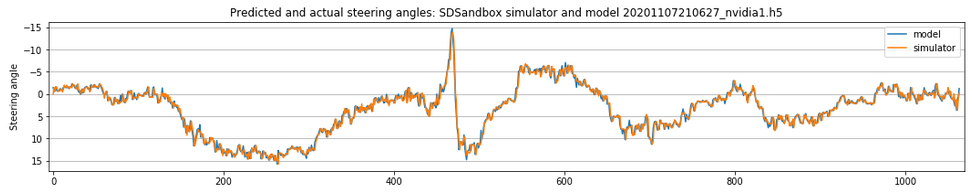
\includegraphics[width=\textwidth]{Figures/PredSteeringAnglestcpflowNvidia1.png}
 \caption{Predicted (blue) and ground-truth simulator (orange) steering angles. The simulator steering angle values in this case are obtained from data packets sent over the TCP network.}
 \label{fig:PredSteeringAnglestcpflowNvidia1}
\end{figure}

Taking this technique one step further, a video can be created using the image sent by simulator, next to the processed image presented to network. Together with the steering angle that would be used by simulator with the steering angle produced by prediction engine (predict\_client.py) which is used by the simulator.

%%%%%%%%%%%%%%%%%%%%%%%%%%%%%%%
% EVALUATIONS ARCHIVED
%%%%%%%%%%%%%%%%%%%%%%%%%%%%%%%

TODO - future work
addressing data imbalance
Binning as an alternative to deep regression models for ResNet, LeNet and VGG net. 
\subsection{Using deep classification models for self-driving CNNs} % Binning/Quantization
Describe this approach, if we get that far, to use an alternative to regression models, whereby we may bin the outputs. This could potentially simplify the model. Also, depending on track, we could have narrower bins around zero degrees, i.e. finer control and wider bins away from zero degrees, i.e. coarser control. Or vice-versa - experimentation required.
\subsection{Data balancing}



%%%%%%%%%%%%%%%%%%%%%%%%%%%%%%%%%%%%%%%%%%%%%%%%%%%%%%%%%%%%%%%%%%%%%%%%%%%%
% On running training on multiple development environments
%%%%%%%%%%%%%%%%%%%%%%%%%%%%%%%%%%%%%%%%%%%%%%%%%%%%%%%%%%%%%%%%%%%%%%%%%%%%
Training models on multiple environments created portability issues because of different version of Python, Keras and Tensorflow, where a model trained on Camber (City cloud service) not running locally. The same was not observed on Intel DevCloud 

TODO - Development environments - need to run same versions of python, keras and tensorflow. Care in setting up environment (potentially virtual) must be taken to ensure models can be run acrsso different machines.
\section{Dropped datasets}
Some effort was expended into downloading datasets and understanding how to extract steering angles from data provided. This drive, together with the expectation of trialing, in addition to variations of DriveNet, ResNet, VGGNet and InceptionNet proved too ambitious.   
%%%%%%%%%%%%%%%%%%%%%%%%%%%%%%%%%%%%%%%%%%%%%%%%
% ALEXNET - NOT READILY IMPLEMENTED IN KERAS
%%%%%%%%%%%%%%%%%%%%%%%%%%%%%%%%%%%%%%%%%%%%%%%%

TODO Add how AlexNet kernel sizes had to be changed in Keras so feature map geometry could be attained. Original Alexnet paper details, as an example, the first kernel dimension as being 11x11 with a stride of 4, with resulting feature maps of size 55x55 in the first convolution layer, the code implementation details were not given. Using the Keras library there was a trade-off between keeping the kernel or the feature map size. To obtain feature maps of 55x55, a kernel of size 8x8 was used, having an effect of the number of trainable parameters. 
Also, the first two fully connected layers with 2048 units each let to compilation errors in Keras (compilation errors left as comments in models.py). The lesson learnt was that network topologies are not readily transferable across libraries, and the description was not sufficient to implement the model in Keras.  

%%%%%%%%%%%%%%%%%%%%%%%%%%%%%%%%%%%%%%%%%%%%%%%%
% DRIVENET - NOT READILY IMPLEMENTED IN KERAS
%%%%%%%%%%%%%%%%%%%%%%%%%%%%%%%%%%%%%%%%%%%%%%%%
The same was observed with DriveNet. One co-author (\ref{urs_muller1}) was very helpful in sharing implementation details not described in the paper. The resulting Keras model failed to produce usable results and had to be modified further, reducing the size of network, as were TawnNet and NaokiNet by their respective authors.



%%%%%%%%%%%%%%%%%%%%%%%%%%%%%%%%%%%%%%%%%%%%%%%%%%%%%%%%%%%%%%%%%%%%%%%%%%%%%%
% On the importance of human readable and self documenting naming conventions
%%%%%%%%%%%%%%%%%%%%%%%%%%%%%%%%%%%%%%%%%%%%%%%%%%%%%%%%%%%%%%%%%%%%%%%%%%%%%%

The naming conventions used in throughout this project, for data directories, models, tcpflow logs, etc, could have benefited from some time invested in searching for a more human-readable and self-documenting scheme, as well as code documentation. An effort was made to this end while the research work was being carried out. Attempts to improve experiment documentation can be seen in \ref{res:training_and_testing_log} where the level of detail and layout increases over time. Still it was laborious sometimes to recall an experiment setup and results, which could be addressed with additional planning.

%%%%%%%%%%%%%%%%%%%%%%%%%%%%%%%%%%%%%%%%%%%%%%%
% Reflections on data imbalance
%%%%%%%%%%%%%%%%%%%%%%%%%%%%%%%%%%%%%%%%%%%%%%%

%%%%%%%%%%%%%%%%%%%%%%%%%%%%%%%%%%%%%%%%%%%%
% TRAINING ENVIRONMENTS
%%%%%%%%%%%%%%%%%%%%%%%%%%%%%%%%%%%%%%%%%%%%
% On cloud environments being slower that local environments
Training environments Camber and Intel DevCloud, although being of a higher specification than the local workstation, proved to be much slower, on account of the shared resources. Jobs ran quicker locally, so over time, Camber and DevCloud were no longer used.


